\chapter{Przegląd literatury oraz projektowanie wieloagentowego systemu opartego na dużych modelach językowych}

Rozwój dużych modeli językowych (LLM) umożliwił powstanie nowej klasy systemów autonomicznych --- agentów zdolnych do samodzielnego planowania, wnioskowania i wykonywania działań w środowiskach wymagających specjalistycznej wiedzy.

Niniejszy rozdział łączy przegląd literatury z opisem autorskiego projektu wieloagentowego systemu autoremediacji. Punktem wyjścia jest paradygmat \textit{Re-Act} oraz analiza jego ograniczeń: limitu okna kontekstowego, degradacji wnioskowania przy długich kontekstach (\textit{Lost in the Middle}) i braku mechanizmów samouczenia. Następnie omówiono architektury wieloagentowe w wariancie \textit{agent-as-a-tool} oraz autorskie rozszerzenia: kompresję kontekstu, hierarchiczny model organizacji pracy oparty na drzewie zadań oraz implementację agenta SRE złożonego z czterech wyspecjalizowanych instancji. Rozdział zamyka opis mechanizmu samouczenia opartego na adaptacji algorytmu \textit{Agentic Context Engineering} (ACE), rozszerzonego o hierarchiczną propagację refleksji wzdłuż drzewa zadań i mechanizmy ograniczania stronniczości.

\section{Agent Re-Act (Reasoning and Acting)}
\subsection{Idea}
\begin{figure}[H]
  \centering
  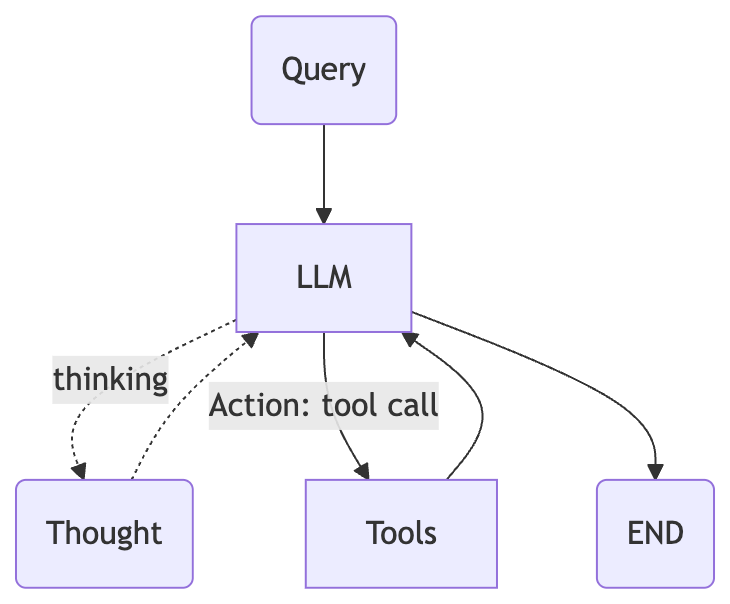
\includegraphics[width=0.5\textwidth]{grafika/re-act-1.png}
  \caption{Schemat agenta Re-Act: na podstawie zapytania agent iteracyjnie myśli lub podejmuje działania z użyciem narzędzi, kończąc pracę, gdy LLM uzna zadanie za wykonane.}
  \label{fig:re-act-1}
\end{figure}
Paradygmat Re-Act, wprowadzony przez Yao i współpracowników \cite{yao2023react}, stanowi fundament współczesnych systemów agentowych opartych na LLM. Łączy on dwa kluczowe procesy:
generowanie śladów rozumowania (\textit{reasoning traces}) oraz wykonywanie specyficznych dla zadania akcji (\textit{acting}). Jak zauważają Sarda i in.
\cite{sarda2024leveraging}, w kontekście autoremediacji mikrousług, podejście to pozwala agentowi nie tylko na wywoływanie narzędzi diagnostycznych, ale przede
wszystkim na werbalizację strategii naprawczej przed jej egzekucją, co znacząco redukuje liczbę błędnych interwencji.
\subsection{Ograniczenia}
Mimo swojej skuteczności i prostoty implementacji, klasyczny agent Re-Act boryka się z istotnymi barierami:
\begin{itemize}
       \item \textbf{Limit okna kontekstowego}: Gromadzenie historii przemyśleń i wyników narzędzi szybko wyczerpuje dostępną pamięć modelu.
       \item \textbf{Degradacja myślenia ("Lost in the Middle")}: Badania Du i in. \cite{du2025context_length_hurts_llm} dowodzą, że sama długość kontekstu negatywniewpływa na zdolność LLM do wnioskowania, nawet przy idealnym systemie wyszukiwania informacji.
       \item \textbf{Limit narzędzi}: Przeciążenie agenta zbyt dużą liczbą dostępnych funkcji prowadzi do halucynacji parametrów lub wyboru nieadekwatnych akcji.
       \item \textbf{Brak mozliwosci samouczenia się}: Agent nie ma mozliwosci wyciagania wniosków z historii konwersacji, co znacząco ogranicza jego zdolność do samouczenia się. 
\end{itemize}

Mimo że obecna architektura modeli LLM nie pozwala na efektywną modyfikację wewnętrznych wag w trakcie działania ani poszerzenie okna kontekstowego, dostępne są techniki \textit{Context Engineering} \cite{mei2025context_engineering_survey}, takie jak RAG \cite{lewis2020rag}, Few-shot Learning \cite{brown2020gpt3} czy GEPA \cite{agrawal2025gepa}, które umożliwiają lepsze wykorzystanie kontekstu i wiedzy modelu bez ingerencji w jego parametry.

\section{Architektura Wieloagentowa}
\subsection{Agent as a Tool}
Współczesne systemy dążą do dekompozycji złożonych problemów na mniejsze, specjalizowane podzadania. Li \cite{li2026single_agent_skills_vs_multiagent} analizuje
dylemat: kiedy pojedynczy agent z bogatym zestawem umiejętności jest lepszy od systemu wieloagentowego. W pracy przyjęto model hybrydowy \textit{Agent as a Tool}.
W tym podejściu, agent nadrzędny traktuje wyspecjalizowane agenty jako narzędzia wywoływane przez dekorator \texttt{@tool}. Pozwala to na:
\begin{itemize}
\item \textbf{Izolację kontekstu}: Każdy pod-agent (np. \textit{Metrics Agent}, \textit{DevOps Agent}, \textit{Incident Commander}) operuje tylko na danych niezbędnych dla jego domeny, zwracając do głównego agenta
jedynie skompresowany wynik (\textit{ToolResult}).
\item \textbf{Niezawodność decyzyjną}: Hierarchiczna struktura pozwala na lepszą weryfikację decyzji na każdym szczeblu, co Lee i in.
\cite{lee2025reliable_multiagent_llm} definiują jako kluczowy element budowania zaufania do systemów autonomicznych.
\end{itemize}
\section{Implementacja Agenta Re-Act - z rekursywną kompresją kontekstu i ograniczeniem iteracji}
Jak wspomniano wcześniej, podstawowa idea \textit{Agenta Re-Act} ma istotne ograniczenia: w przypadku złożonych, nieprzewidywalnych zadań liczba iteracji może gwałtownie wzrosnąć, co prowadzi do przepełnienia okna kontekstowego, pogorszenia wnioskowania i uniemożliwia dalsze działanie agenta (np. po wczytaniu zbyt wielu wpisów z logów). Dlatego w niniejszej implementacji wprowadzono dwa kluczowe mechanizmy: (1) automatyczną kontrolę rozmiaru okna kontekstowego i w razie potrzeby uruchamianie jego kompresji, oraz (2) limit iteracji – po jego przekroczeniu agent tworzy podsumowanie dotychczasowych działań i kończy pracę. Pozwala to zachować efektywność agenta nawet w niestandardowych scenariuszach.


\begin{figure}[H]
    \centering
    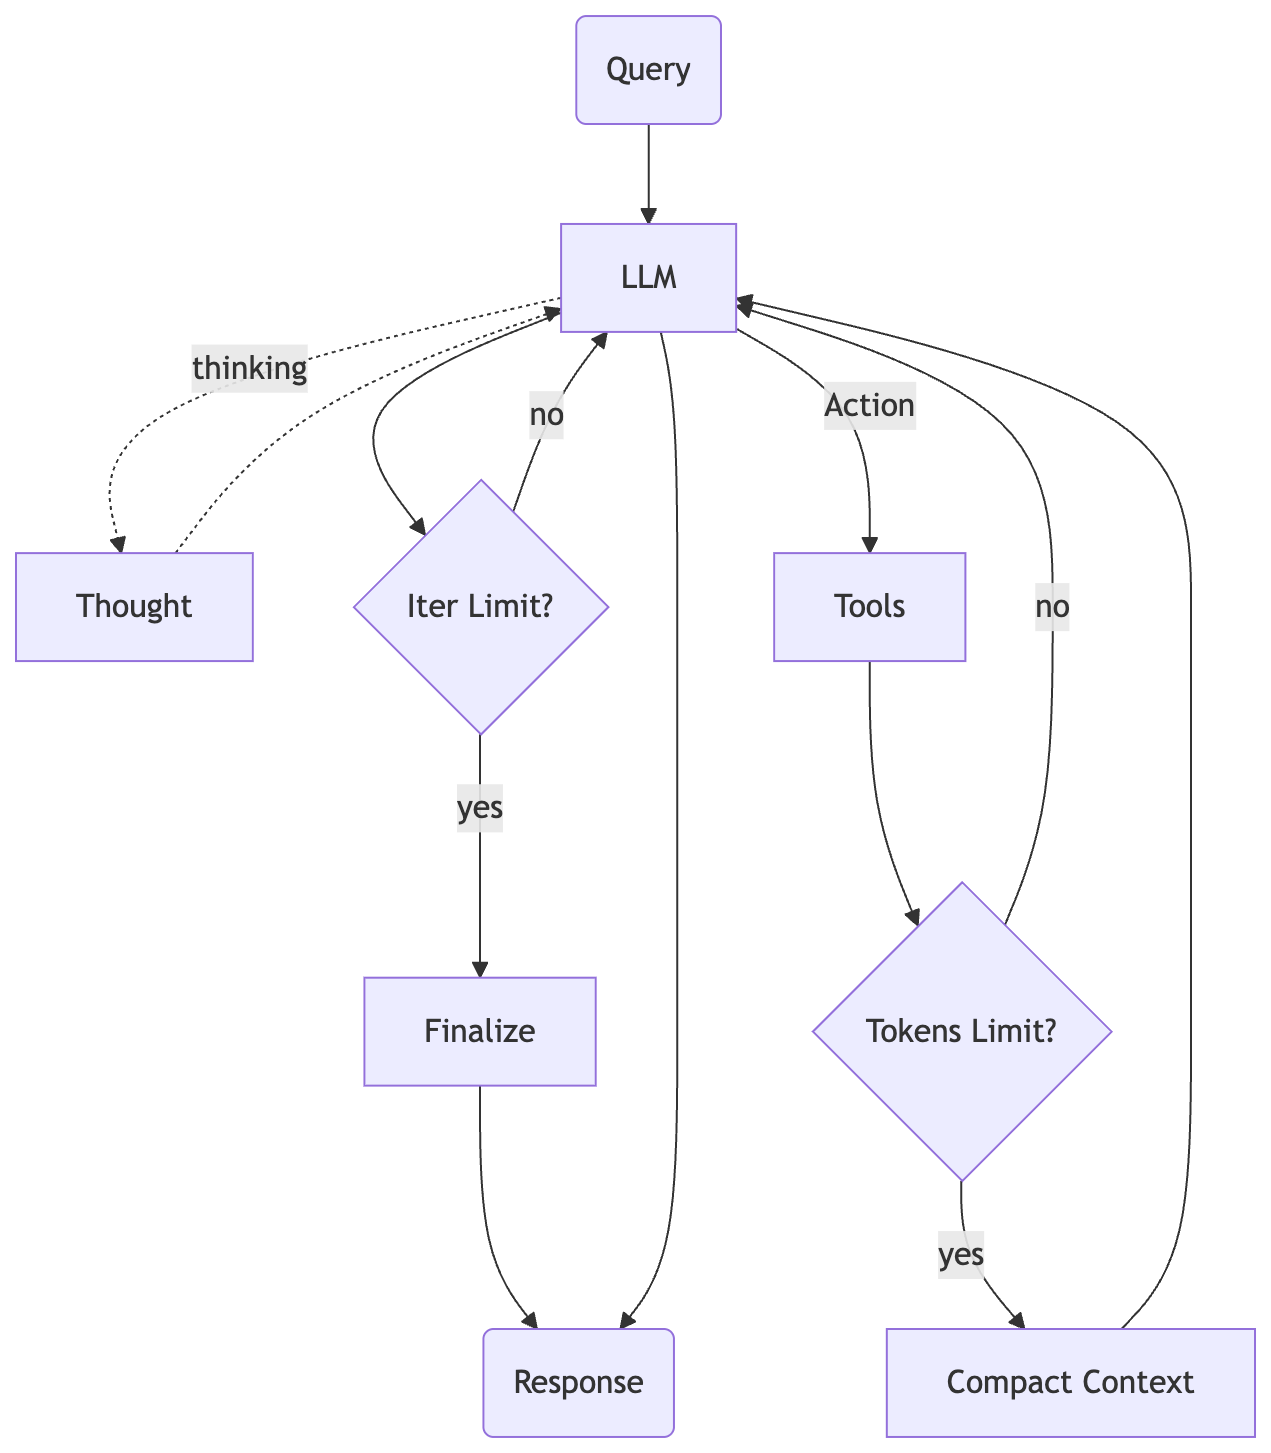
\includegraphics[width=0.5\textwidth]{grafika/re-act-2.png}
    \caption{Agent Re-Act: kompresja kontekstu i limit iteracji (schemat implementacji).}
    \label{fig:re-act-2}
\end{figure}

\begin{algorithm}[H]
    \scriptsize
    \SetAlgoLined
    \DontPrintSemicolon
    \KwData{Zapytanie $Q$, limit iteracji $N$, próg tokenów $T$}
    $C \leftarrow Q$, $i \leftarrow 0$\;
    \While{$i<N$}{
        $i\leftarrow i+1$\; 
        $A \leftarrow \text{LLM}(C)$\;
        \If{Odpowiedź końcowa $\in A$}{\Return $A$}
        $O \leftarrow \text{WykonajNarzędzia}(A)$\;
        \If{$\text{PoliczTokeny}(O)>T$}{$O \leftarrow \text{Kompresja}(O)$}
        $C \leftarrow C \cup \{A,O\}$\;
    }
    \Return{\text{Zakończ}($C$)}
    \caption{\scriptsize Agent Re-Act z kompresją kontekstu i limitem iteracji}
\end{algorithm}

\subsection{Kompresja kontekstu}
Gdy szacowana liczba tokenów w historii konwersacji osiąga próg z konfiguracji modelu, uruchamiana jest kompresja: starsza część dialogu jest zastępowana tekstowym podsumowaniem wygenerowanym przez osobne wywołanie LLM. W~konfiguracji próg ten wynosi około 64~tys.\ tokenów przy oknie kontekstowym 200~tys.\ tokenów, co odpowiada około 32\% dostępnego okna i~ogranicza narastanie historii wtedy, gdy długość kontekstu mogłaby obniżyć jakość rozumowania agenta.

Domyślnie do kompresji stosuje się specjalnie przygotowany prompt systemowy wymagający uporządkowanego streszczenia (m.in.\ dotychczasowy tok rozmowy, bieżąca praca, pojęcia techniczne, pliki i~fragmenty kodu, rozwiązane problemy oraz oczekujące kroki). Na końcu żądania dokładana jest krótka wiadomość użytkownika prosząca o~podsumowanie zgodnie z tą instrukcją. Przy wielokrotnej kompresji, jeśli w historii występuje już wcześniejsze podsumowanie, dołączana jest prośba o kontynuację od podanego streszczenia.
\newpage
Pełna treść domyślnego promptu systemowego (pochodząca z projektu Roo Code \cite{roocode_github}) oraz komunikatów pomocniczych przedstawiono w~listingach~\ref{lst:summary-prompt}--\ref{lst:continue-summary}.

\begin{lstlisting}[basicstyle=\footnotesize\ttfamily,breaklines=true,columns=fullflexible]
Your task is to create a detailed summary of the conversation so far, paying close attention to the user's explicit requests and your previous actions.
This summary should be thorough in capturing technical details, code patterns, and architectural decisions that would be essential for continuing with the conversation and supporting any continuing tasks.

Your summary should be structured as follows:
Context: The context to continue the conversation with. If applicable based on the current task, this should include:
  1. Previous Conversation: High level details about what was discussed throughout the entire conversation with the user. This should be written to allow someone to be able to follow the general overarching conversation flow.
  2. Current Work: Describe in detail what was being worked on prior to this request to summarize the conversation. Pay special attention to the more recent messages in the conversation.
  3. Key Technical Concepts: List all important technical concepts, technologies, coding conventions, and frameworks discussed, which might be relevant for continuing with this work.
  4. Relevant Files and Code: If applicable, enumerate specific files and code sections examined, modified, or created for the task continuation. Pay special attention to the most recent messages and changes.
  5. Problem Solving: Document problems solved thus far and any ongoing troubleshooting efforts.
  6. Pending Tasks and Next Steps: Outline all pending tasks that you have explicitly been asked to work on, as well as list the next steps you will take for all outstanding work, if applicable. Include code snippets where they add clarity. For any next steps, include direct quotes from the most recent conversation showing exactly what task you were working on and where you left off. This should be verbatim to ensure there's no information loss in context between tasks.

Example summary structure:
1. Previous Conversation:
  [Detailed description]
2. Current Work:
  [Detailed description]
3. Key Technical Concepts:
  - [Concept 1]
  - [Concept 2]
  - [...]
4. Relevant Files and Code:
  - [File Name 1]
    - [Summary of why this file is important]
    - [Summary of the changes made to this file, if any]
    - [Important Code Snippet]
  - [File Name 2]
    - [Important Code Snippet]
  - [...]
5. Problem Solving:
  [Detailed description]
6. Pending Tasks and Next Steps:
  - [Task 1 details \& next steps]
  - [Task 2 details \& next steps]
  - [...]

Output only the summary of the conversation so far, without any additional commentary or explanation.
\end{lstlisting}
\captionof{lstlisting}{Domyślny prompt systemowy \texttt{SUMMARY\_PROMPT} używany przy kompresji kontekstu (\texttt{agent/context\_ops.py}).}
\label{lst:summary-prompt}

\begin{lstlisting}[basicstyle=\footnotesize\ttfamily,breaklines=true,columns=fullflexible]
Summarize the conversation so far, as described in the prompt instructions.
\end{lstlisting}
\captionof{lstlisting}{Końcowa wiadomość użytkownika dołączana do żądania podsumowania (\texttt{final\_request\_message}, \texttt{agent/context\_ops.py}).}
\label{lst:condense-final}

\begin{lstlisting}[basicstyle=\footnotesize\ttfamily,breaklines=true,columns=fullflexible]
Please continue from the following summary:
\end{lstlisting}
\captionof{lstlisting}{Treść wiadomości użytkownika wstawianej przy kontynuacji od wcześniejszego streszczenia (\texttt{get\_messages\_since\_last\_summary}, \texttt{agent/context\_ops.py}).}
\label{lst:continue-summary}
\section{Organizacja oraz Koordynacja Wieloagentowa}

Efektywność systemów wieloagentowych w kontekście skomplikowanych zadań silnie zależy od spójnych mechanizmów delegacji i koordynacji pracy agentów. W eksperymentach z amorficznymi, niehierarchicznymi strukturami rozproszonymi napotkano trudności z harmonijną współpracą, dlatego postawiono na hierarchiczny model z drzewem zadań (\textit{tasks tree}), który zapewnia jasność podziału obowiązków oraz skuteczne zarządzanie przepływem pracy.

Inspiracją dla tej architektury były praktyki stosowane m.in. przez Asanę w modelu \textit{WorkGraph}, w którym Agent AI wykorzystuje strukturę drzewa zadań do koordynacji pracy agentów\cite{asana_work_graph, asana_ai_teammates_2024}, podobne implementacje są równiez stosowane w projektach takich jak Roo-Code \cite{roocode_github}. W naszym rozwiązaniu centralną rolę pełni \textit{Incident Commander}, który koordynuje prace agentów wyspecjalizowanych, takich jak \textit{Metrics Agent}, \textit{DevOps Agent}, czy \textit{Coder Agent}.

\subsection{Hierarchia i Drzewo Zadań}

Wielopoziomowa struktura organizacyjna bazuje na drzewie zadań – główny agent rozkłada ogólny cel na spójne podzadania i przydziela je agentom podrzędnym, dbając przy tym o zależności i kolejność realizacji. Taki układ ułatwia zarówno śledzenie postępu, jak i zapewnienie spójności oraz przejrzystości działań w ramach całego systemu.

\begin{figure}[H]
    \centering
    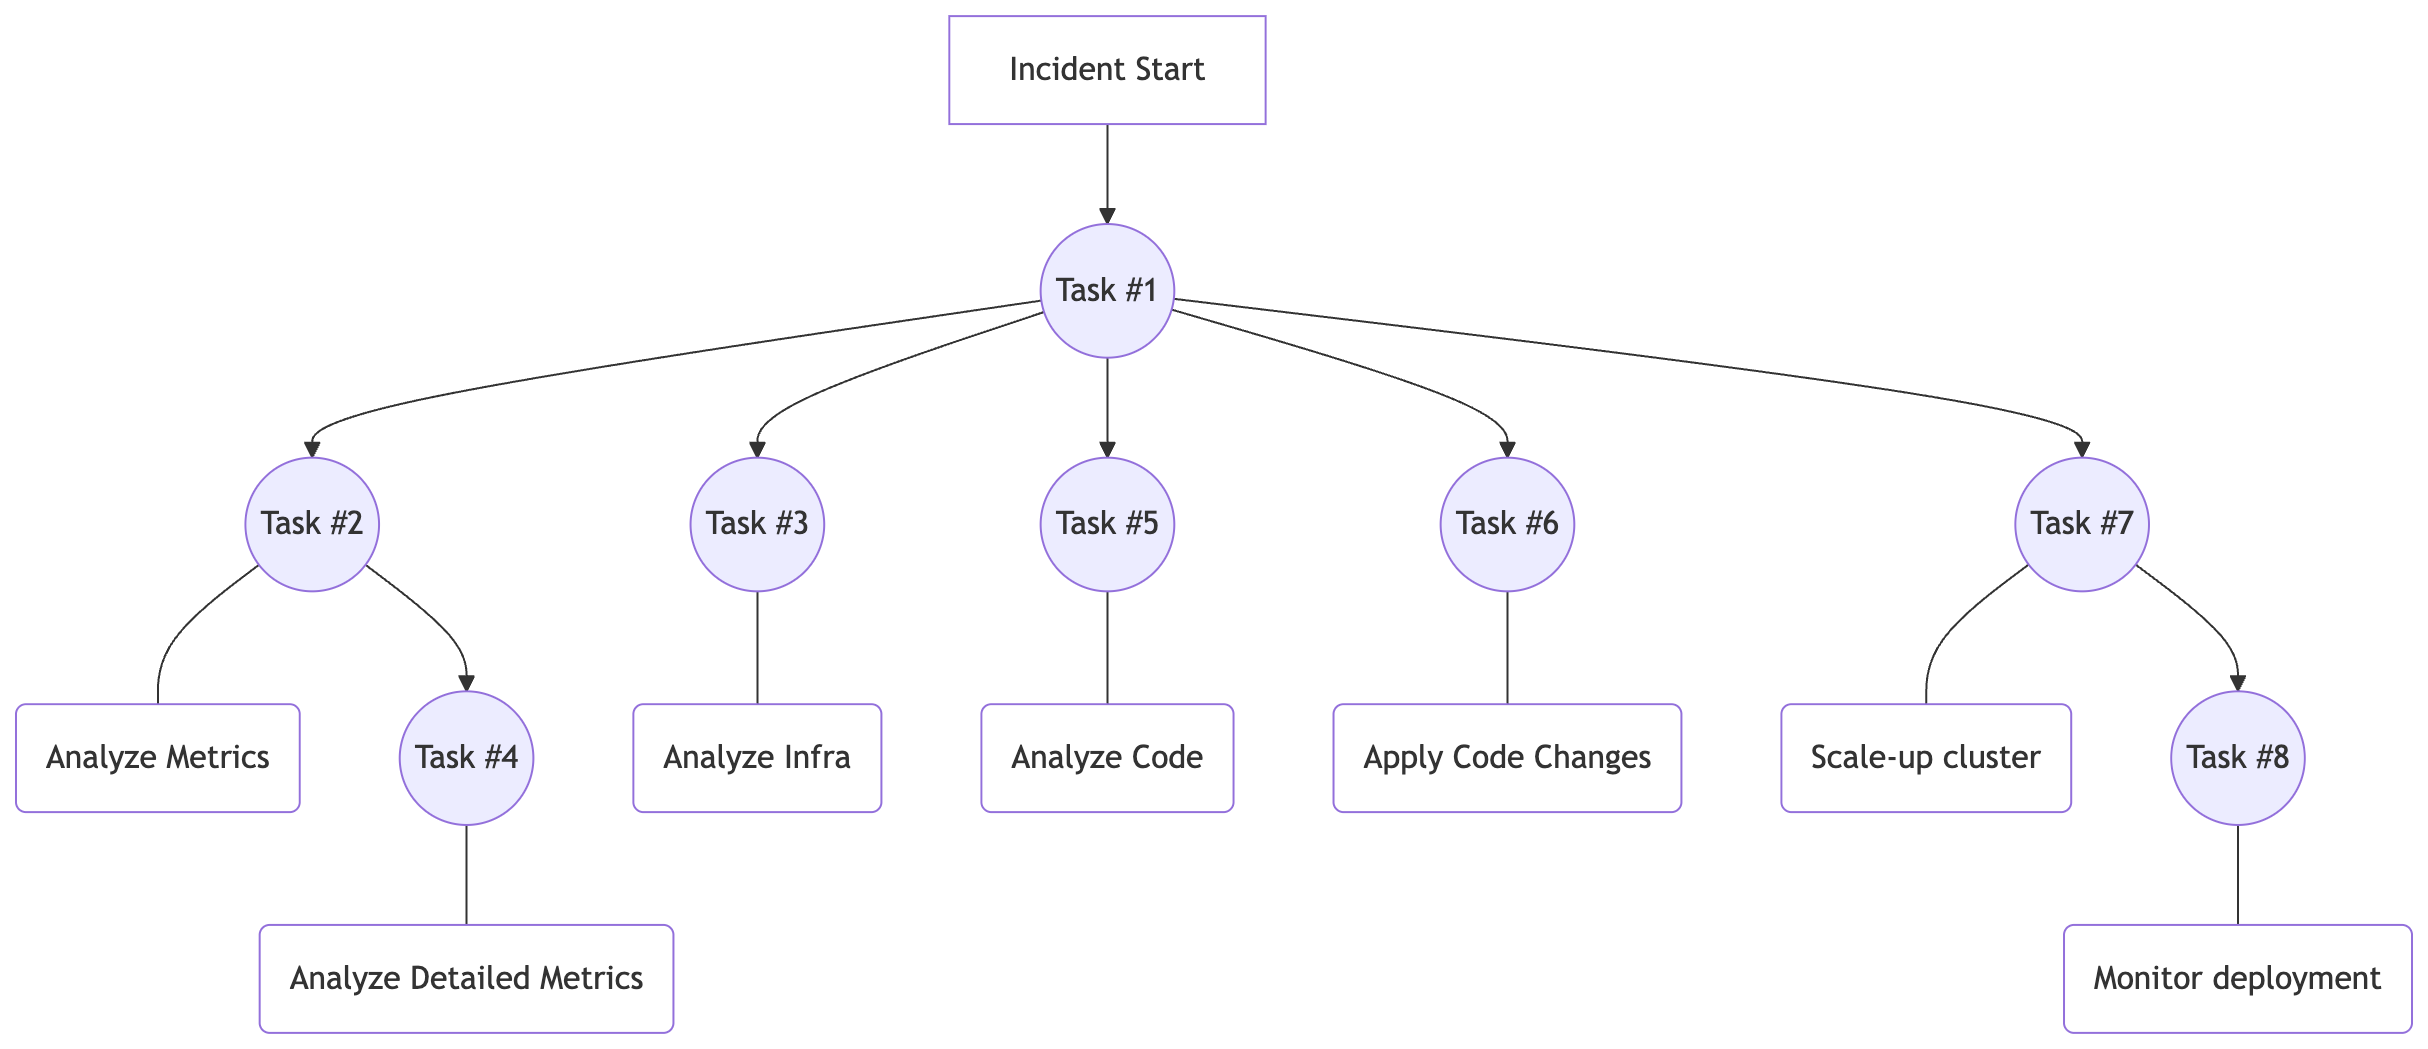
\includegraphics[width=\textwidth]{grafika/tasks-tree.png}
    \caption{Schemat drzewa zadań: główny agent rozbija cel nadrzędny na powiązane podzadania, deleguje je agentom podrzędnym, a zależności pomiędzy zadaniami odzwierciedlają zarówno hierarchię, jak i koordynację pracy.}
    \label{fig:tasks-tree}
\end{figure}

\subsection{Delegacja, Egzekucja i Komunikacja Agentów}

Delegowanie, realizacja i egzekwowanie zadań w systemie agentskim są wspierane poprzez wyraźnie zdefiniowane narzędzia operacyjne, takie jak \texttt{assign\_task}, \texttt{update\_todo} i \texttt{provide\_feedback}. Umożliwiają one tworzenie podzadań, monitorowanie postępów, a także wymianę informacji zwrotnej między agentami, co usprawnia całą współpracę.

Proces przebiega iteracyjnie i obejmuje następujące etapy:

\begin{enumerate}
  \item \textbf{Inicjacja podzadania}: Główny agent przekazuje cel, kroki realizacji i kontekst wybranemu wykonawcy.
  \item \textbf{Wykonanie}: Podwykonawca przystępuje do pracy, realizując zadanie według przekazanej specyfikacji i aktualizując status na bieżąco.
  \item \textbf{Weryfikacja i feedback}: Każde zakończone podejście jest oceniane przez agenta zlecającego – otrzymuje on możliwość zatwierdzenia, odrzucenia lub przekazania wskazówek do poprawek.
  \item \textbf{Iteracja}: W razie konieczności, zadanie powtarzane jest do momentu osiągnięcia określonego efektu lub wyczerpania limitu prób.
  \item \textbf{Finalizacja}: Zadanie zostaje zakończone po pozytywnej ocenie lub odrzucone, gdy cele nie są osiągalne.
\end{enumerate}

Dzięki powyższemu podejściu możliwa jest precyzyjna kontrola procesu, przejrzysty monitoring postępu, a także wielokrotna iteracja rozwiązań – co odzwierciedla rzeczywistą współpracę zespołową również w rozbudowanych, zagnieżdżonych strukturach.

\begin{figure}[H]
    \centering
    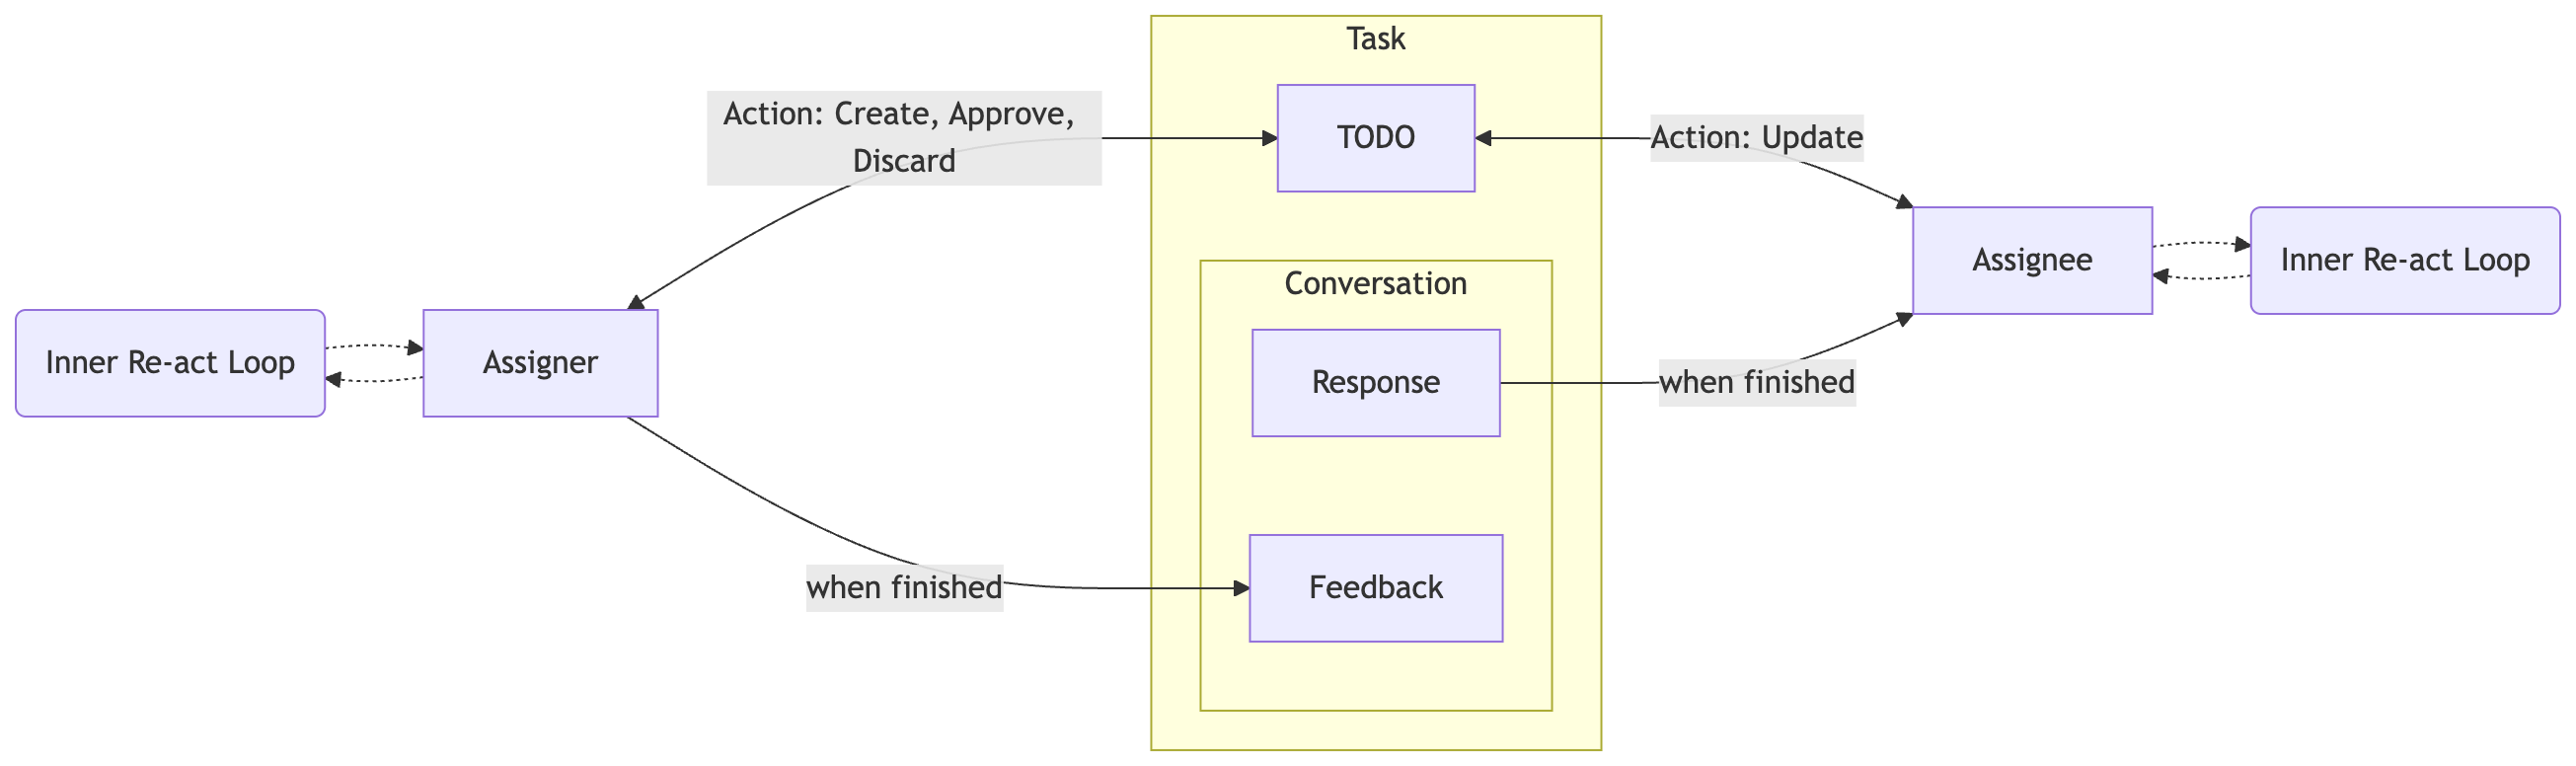
\includegraphics[width=\textwidth]{grafika/task-conversation.png}
    \caption{Konwersacja oraz egzekucja zadania: główny agent dzieli cel na podzadania i deleguje je agentom, nadzorując całość procesu oraz weryfikując rezultaty.}
    \label{fig:tasks-conversation}
\end{figure}

Praktyczna implementacja tego modelu znajduje się w modułach \texttt{agent/tasks/executor.py} oraz~\texttt{agent/tooling/planning.py}.

\section{Implementacja Agenta SRE}

\begin{figure}[H]
    \centering
    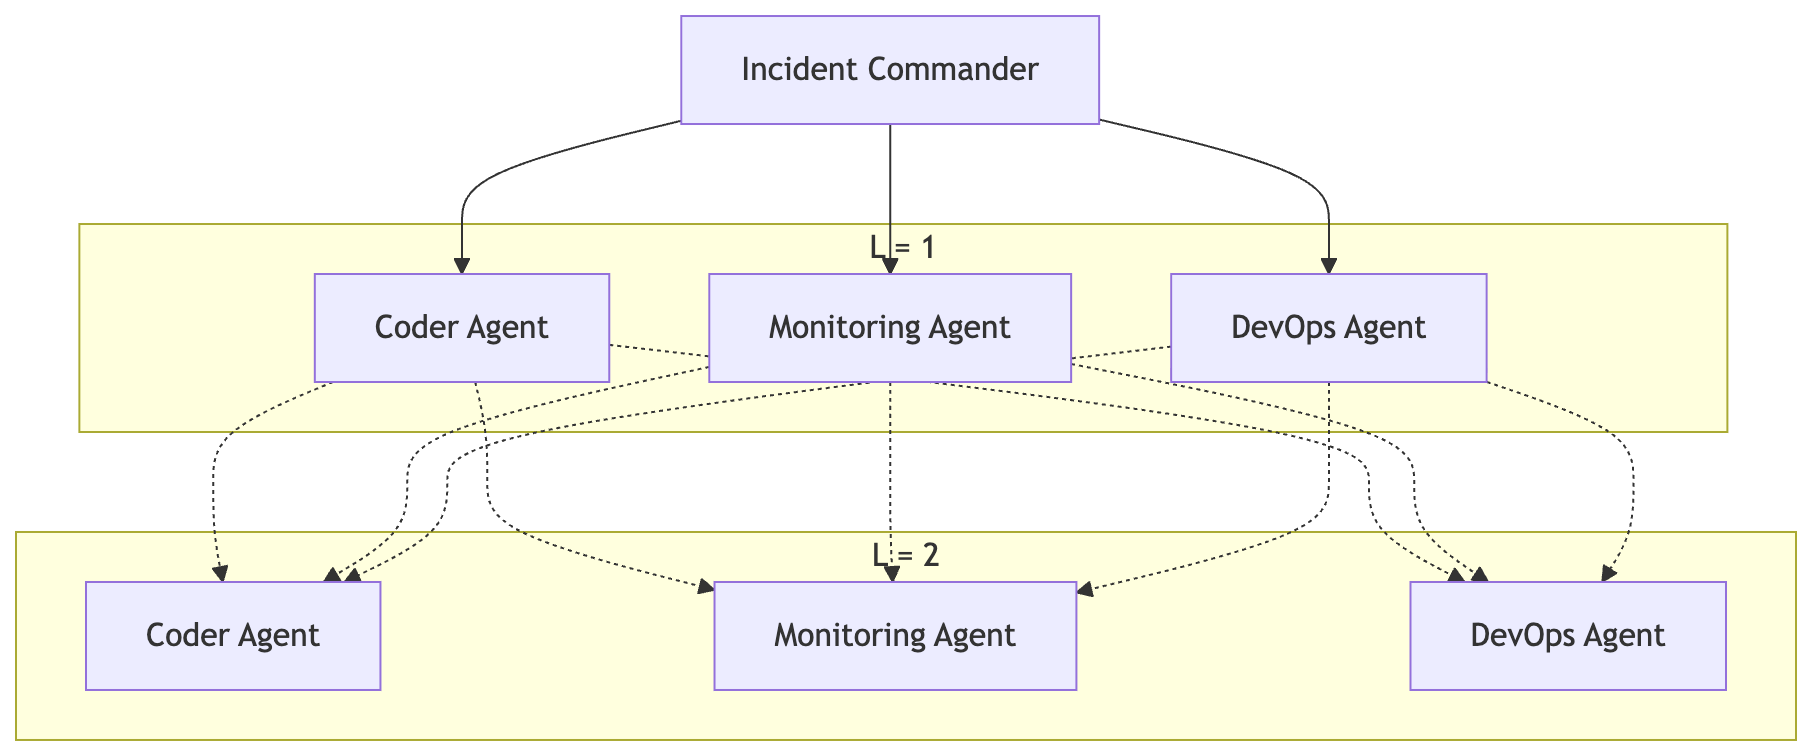
\includegraphics[width=\textwidth]{grafika/sre-agent.png}
    \caption{Schemat implementacji agenta SRE: \textit{Incident Commander} koordynuje prace agentów wyspecjalizowanych, takich jak \textit{Metrics Agent}, \textit{DevOps Agent}, czy \textit{Coder Agent}. Każdy z agentów może delegować zadania innym agentom, a także wywoływać narzędzia operacyjne. Wysokość drzewa została ograniczona do 3 poziomów (\textit{Incident Commander}(\textit{L0}) -> \textit{L1} -> \textit{L2}), aby uniknąć zdbyt głębokiej rekursji.}
    \label{fig:sre-agent}
\end{figure}

W warstwie implementacji agent SRE jest konfigurowany jako grupa czterech instancji — komendanta \textit{Incident Commander}, agenta metryk \textit{Metrics Agent}, DevOps \textit{DevOps Agent} oraz agenta kodu \textit{Coder Agent} — z różnymi zestawami narzędzi i ze wspólnym kontekstem: katalogiem roboczym, klientem API Grafana oraz zmiennymi środowiskowymi AWS wykorzystywanymi przy operacjach na klastrze. Koordynacja zadań opiera się na jasno określonych mechanizmach delegowania, aktualizowania zadań i egzekwowania ich realizacji, zgodnie z opisem w podrozdziale o delegacji.

\subsection{Incident Commander}

\textit{Incident Commander} jest agentem nadrzędnym: w promptcie systemowym ma wskazanych deputatów (\texttt{coder\_agent}, \texttt{monitoring\_agent}, \texttt{devops\_agent}) oraz obowiązek uruchomienia wdrożenia po przygotowaniu poprawki. Jego zestaw narzędzi ograniczono do planowania oraz~\texttt{deploy\_app} — wywołania skryptu powłoki (np.\ \texttt{deploy.sh}) wdrażającego aplikację w~Kubernetes, z~przekazaną ścieżką i~środowiskiem w~kontekście. Komendant nie otrzymuje bezpośredniego dostępu do poleceń \texttt{kubectl}, edycji kodu ani zapytań do metryk; jego rola to rozdzielenie pracy i~finalne wdrożenie.

\subsection{Metrics Agent}

Agent metryk (\texttt{monitoring\_agent}) został rozbudowany o paradygmat \textit{Recursive Language Models} (RLM) \cite{rlm}, co pozwala na analizę obszernych zbiorów danych obserwowalności bez ryzyka degradacji jakości odpowiedzi wynikającej z przepełnienia okna kontekstowego. Zamiast przesyłać surowe logi bezpośrednio do modelu, agent wykorzystuje izolowane środowisko wykonawcze Python (\texttt{ContainerRLMSandbox}) oraz dedykowanego klienta \texttt{GrafanaPandasClient}. Podejście to umożliwia programowe pobieranie danych z systemów Prometheus i Loki bezpośrednio do struktur \texttt{pandas.DataFrame}, ich agregację, filtrowanie oraz detekcję wzorców (ang. \textit{pattern-matching}) na poziomie kodu. Wyniki analizy mogą być wymieniane między agentami poprzez współdzielony wolumen (\textit{handover volume}), co wspiera wieloetapowe wnioskowanie o przyczynach źródłowych (ang. \textit{root-cause analysis}). Agent posiada również dostęp do narzędzi \texttt{MetricsSummaryTools}, \texttt{kubectl\_get\_resources} oraz funkcji planistycznych, co czyni go autonomicznym analitykiem danych SRE, zdolnym do obsługi incydentów o wysokiej złożoności danych.

\subsection{DevOps Agent}

\textit{DevOps Agent} (\texttt{devops\_agent}) posiada najszerszy zestaw narzędzi: odczyt i~zapis w~klastrze (\texttt{KubectlReadTools}, \texttt{KubectlWriteTools}), operacje na zasobach EKS (\texttt{EksReadTools}, \texttt{EksWriteTools}), powłoka (\texttt{CliTools}) oraz przegląd i~modyfikacja kodu w~przestrzeni roboczej (\texttt{CodebaseReadTools}, \texttt{CodebaseWriteTools}), uzupełnione o~planowanie. Prompt systemowy kieruje uwagę na przestrzeń nazw, w~której działa aplikacja. Agent może delegować m.in.\ do agenta metryk lub wywoływać siebie rekurencyjnie przy złożonych podzadaniach operacyjnych.

\section{Samouczenie się}

Implementacja mechanizmu ewolucji wiedzy w systemie opiera się na paradygmacie \textit{Agentic Context Engineering} (ACE), zaproponowanym przez Zhanga i współpracowników \cite{zhang2025agentic_context_engineering}. Algorytm ten został w niniejszej pracy istotnie rozszerzony i dostosowany do specyfiki hierarchicznej architektury wieloagentowej typu \textit{agent-as-a-tool}. Zamiast tradycyjnego douczania wag modelu (\textit{fine-tuning}), system optymalizuje swoje działanie poprzez ciągłą ewolucję zewnętrznego kontekstu operacyjnego --- tzw. Playbooka.

\begin{figure}[H]
  \centering
  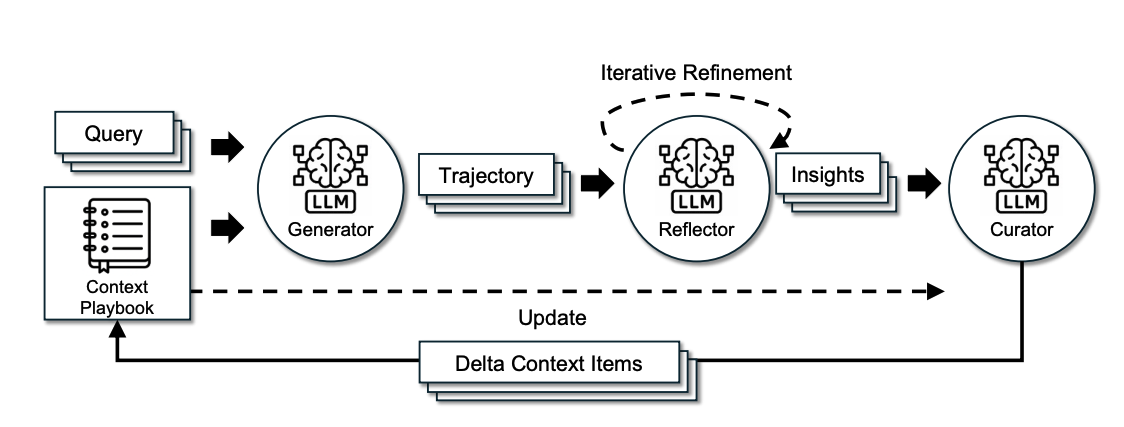
\includegraphics[width=1\textwidth]{grafika/ace-idea.png}
  \caption{Schemat ideii przepływu z publikacji \textit{Agentic Context Engineering: Evolving Contexts for Self-Improving Language Models} \cite{zhang2025agentic_context_engineering}, agent wykonujący pracę generuje trajektorie (ciągi myśli i akcji). \textit{Reflektor} ocenia przebieg pracy (trajektorie) i dzieli się refleksjami z \textit{Kuratorem}, który na ich podstawie wprowadza zmiany do \textit{Playbooka}}
  \label{fig:ace-idea}
\end{figure}

Centralnym elementem potoku ACE (szczegółowo zaimplementowanego w modułach \texttt{ace/pipeline.py} oraz \texttt{ace/playbook\_core.py}) jest iteracyjny proces zbierania doświadczeń z zakończonych zadań, ich krytycznej analizy oraz syntezy nowych reguł. Proces ten realizowany jest przez wyspecjalizowane agenty:

\begin{itemize}
  \item \textbf{Reflector} (\textit{Reflektor}) -- agent diagnostyczny, którego zadaniem jest retrospektywna analiza śladu wykonania zadania (\textit{trace analysis}). Porównuje on podjęte przez agenta SRE kroki z ostatecznym wynikiem (sukcesem lub porażką) i identyfikuje tzw. "Moment Dywergencji" --- punkt, w którym strategia odbiegła od optymalnej. Szablon instrukcji dla tego agenta przedstawiono na rysunku \ref{fig:reflector-prompt}.
  \item \textbf{Curator} (\textit{Kurator}) -- architekt wiedzy, który na podstawie zbioru refleksji podejmuje decyzje o modyfikacji Playbooka (operacje ADD, UPDATE, DELETE). Kryteria decyzyjne kuratora zawarte są w jego prompcie systemowym (rys. \ref{fig:curator-prompt}).
\end{itemize}

\begin{figure}[H]
    \centering
    \lstinputlisting[basicstyle=\tiny\ttfamily, frame=single, breaklines=true, label={fig:reflector-prompt}, caption={Szablon promptu systemowego dla Reflektora Agenta SRE}]{grafika/reflector-prompt-template.md}
\end{figure}

\begin{figure}[H]
    \centering
    \lstinputlisting[basicstyle=\tiny\ttfamily, frame=single, breaklines=true, label={fig:curator-prompt}, caption={Szablon promptu systemowego dla Kuratora Agenta SRE}]{grafika/curator-prompt-template.md}
\end{figure}

\subsection{Analiza refleksji i przyrostowa budowa wiedzy}

Wynikiem pracy Reflektora jest ustrukturyzowany raport (rys. \ref{fig:reflection-example}), który zawiera nie tylko ocenę istniejących punktów Playbooka, ale przede wszystkim tzw. \textit{playbook\_amendment} --- propozycję nowej reguły w formacie IF/THEN oraz \textit{useful\_facts} --- zweryfikowane fakty o architekturze systemu odkryte podczas diagnozy.

\begin{figure}[H]
    \centering
    \lstinputlisting[basicstyle=\tiny\ttfamily, frame=single, breaklines=true, label={fig:reflection-example}, caption={Przykład wygenerowanej refleksji po incydencie typu "Performance Degradation".}]{grafika/reflection-example.md}
\end{figure}

\subsection{Unikanie stronniczości i rola parametrów feedbacku}

W celu zapewnienia obiektywności procesu uczenia, w architekturze wprowadzono mechanizm separacji danych dotyczących skuteczności reguł. Każdy punkt w Playbooku (\textit{bullet}) posiada przypisane parametry \texttt{helpful} oraz \texttt{harmful}, inkrementowane przez Reflektora na podstawie analizy konkretnych incydentów. 

Kluczowym usprawnieniem względem bazowego algorytmu ACE jest \textbf{ukrywanie tych wag przed samym agentem SRE oraz agentem Reflector}. Zapobiega to występowaniu stronniczości (\textit{bias}): agent wykonawczy nie faworyzuje reguł o wysokiej punktacji kosztem nowych propozycji, a Reflektor ocenia przydatność reguły wyłącznie na podstawie bieżącego śladu wykonania, a nie jej historycznej popularności. Pełny wgląd w statystyki (\textit{harmful}, \textit{helpful}) posiada wyłącznie agent \textbf{Curator}, co pozwala mu na podejmowanie racjonalnych decyzji o usunięciu reguł, które w dłuższej perspektywie okazują się szkodliwe lub nieefektywne.

    \begin{figure}[H]
        \centering
        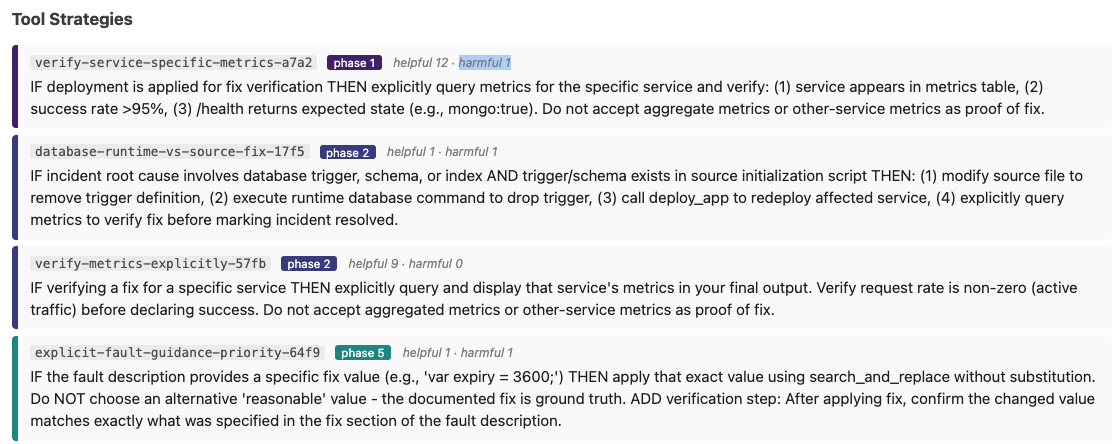
\includegraphics[width=\textwidth]{grafika/playbook_example_with_points.png}
        \caption{Fragment Playbooka dotyczący strategii używania narzędzi, z punktacją \textit{harmful/helpful} i oznaczeniem faz w której zostały dodane punkty.}
    \label{fig:playbook-points}
\end{figure}

\subsection{Hierarchiczna propagacja refleksji}

W przeciwieństwie do systemów jednoagentowych, w przyjętej architekturze refleksje są generowane i przekazywane wzdłuż drzewa zadań. Mechanizm \texttt{reflect\_on\_assignment} pozwala na sytuację, w której agent nadrzędny (np. \textit{Incident Commander}), analizując wynik delegowanego zadania, generuje refleksję skierowaną bezpośrednio do agenta podrzędnego (np. \textit{DevOps Agent}). 

Taki przepływ informacji pozwala na precyzyjne adresowanie błędów w komunikacji i delegacji --- Reflektor może zidentyfikować, że przyczyną niepowodzenia nie był brak umiejętności podwykonawcy, lecz nieprecyzyjne instrukcje przekazane przez zleceniodawcę. Refleksje te są następnie agregowane przez potok ACE i integrowane z Playbookami odpowiednich ról, co prowadzi do spójnego rozwoju kompetencji całego systemu.

\begin{figure}[H]
    \centering
    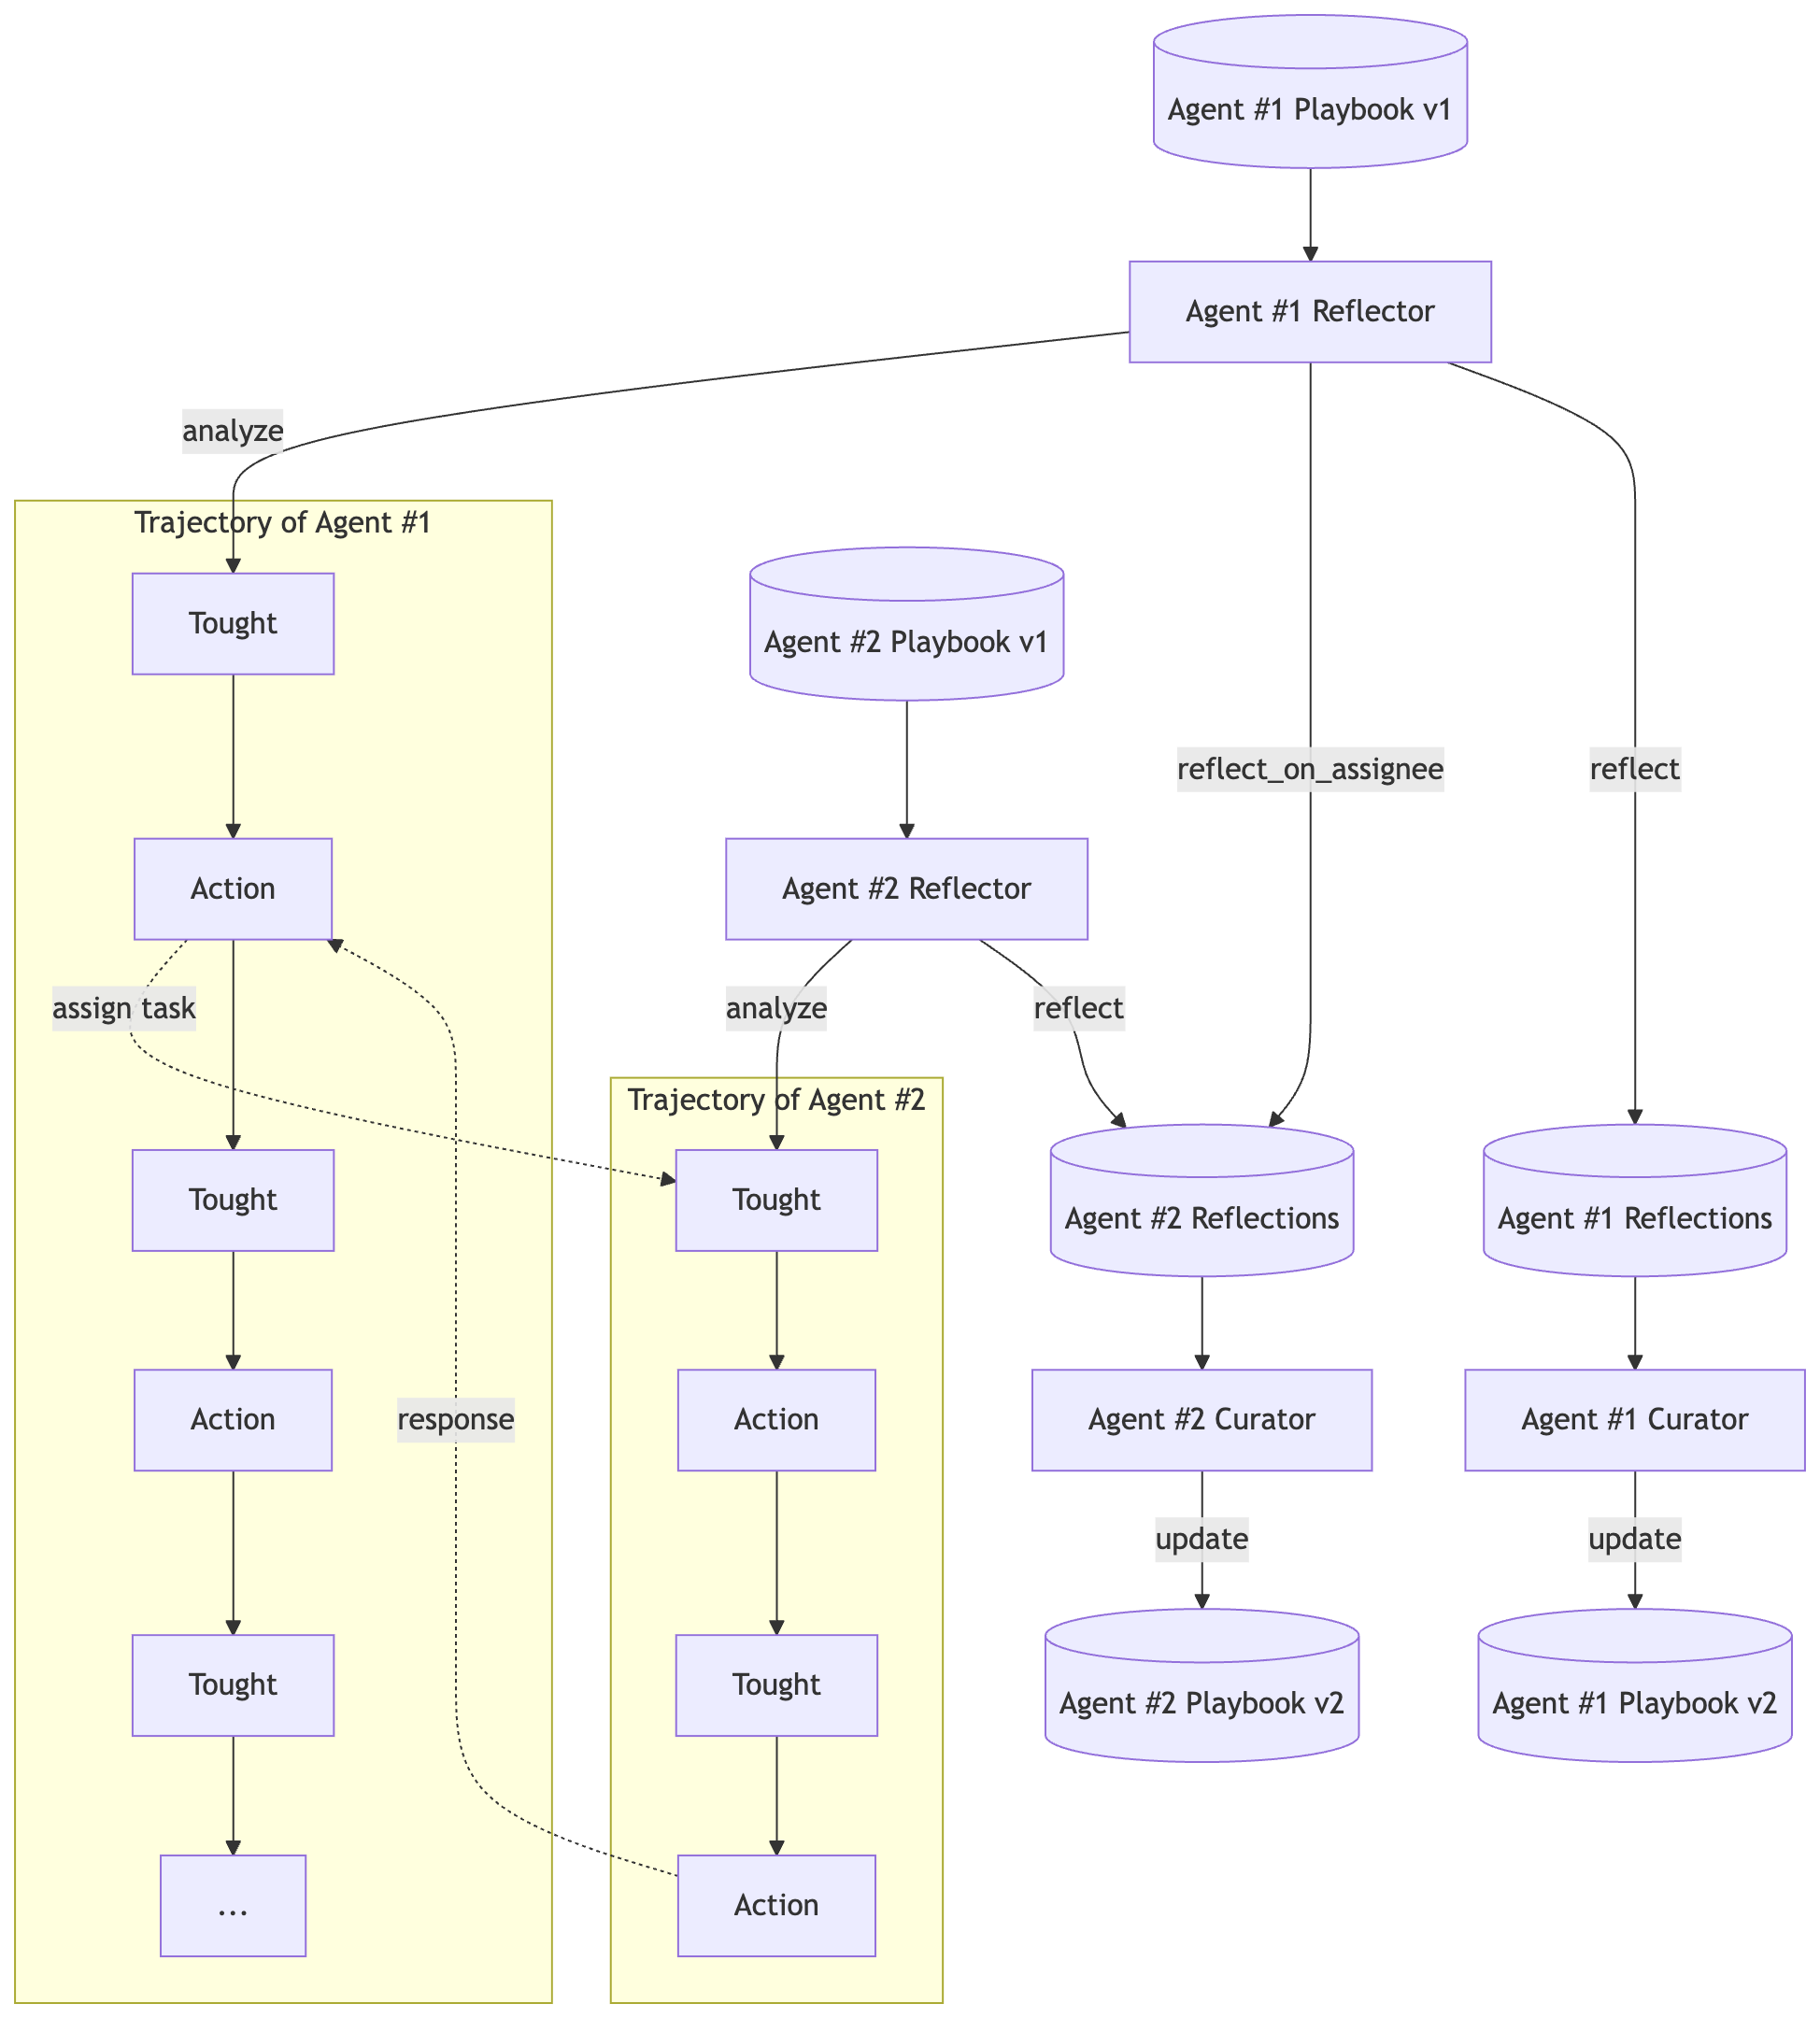
\includegraphics[width=1\textwidth]{grafika/multiagent-ace.png}
    \caption{Schemat ACE Pipeline dla architektury wieloagentowej. Reflektor przypisany do Agenta~1 analizuje pełną trajektorię – obejmującą zarówno własne akcje, jak i działania delegowane. W rezultacie powstaje kolekcja refleksji adresowanych do Agenta~1 oraz Agenta~2 (wykonawcy podzadania). Następnie Kurator, w oparciu o zebrane refleksje, aktualizuje odpowiednie playbooki, zapewniając ciągłą ewolucję wiedzy operacyjnej całego systemu.}
    \label{fig:multiagent-ace}
\end{figure}

\subsection{Wstrzykiwanie wyuczonego kontekstu do agenta SRE}

Samouczenie zgodnie z ACE dotyczy treści operacyjnej (playbook), a nie wag modelu. W architekturze wieloagentowej heurystyki te są dynamicznie dołączane do systemowego promptu każdej instancji agenta na podstawie słownika playbooków, gdzie klucze odpowiadają przypisanym rolom. Dzięki temu podczas kolejnych epizodów autoremediacji agenci – zarówno główny, jak i wyspecjalizowani – korzystają już z wiedzy pozyskanej w ramach potoku ACE.



